\documentclass{article}
\usepackage{newtxtext}
\usepackage{newtxmath}

\usepackage{booktabs} % for better looking tables
\usepackage{graphicx}
\usepackage{caption} % for customizing captions
\usepackage[table]{xcolor} % for coloring tables
\usepackage{pdflscape} % for landscape orientation
\usepackage{arydshln} % for dotted lines in tables	
\usepackage{adjustbox} % For adjusting table position
\usepackage{siunitx}
\usepackage{amsmath}
\usepackage{rotating}
\usepackage{lscape}
\usepackage{multirow}
%\usepackage{geometry}
\usepackage{hhline} % for bold lines
\usepackage{appendix} % for appendix numbering

\begin{document}
\thispagestyle{empty} % Remove page number from this page

\noindent
FIGURES AND TABLES TO: \newline
CORPORATE DEMOGRAPHY AND WAGE INEQUALITY: REVISITED\newline
2024-05-28

\clearpage % Start a new page
\thispagestyle{empty} % Remove page number from this page

\begin{figure}[htbp]
  \centering

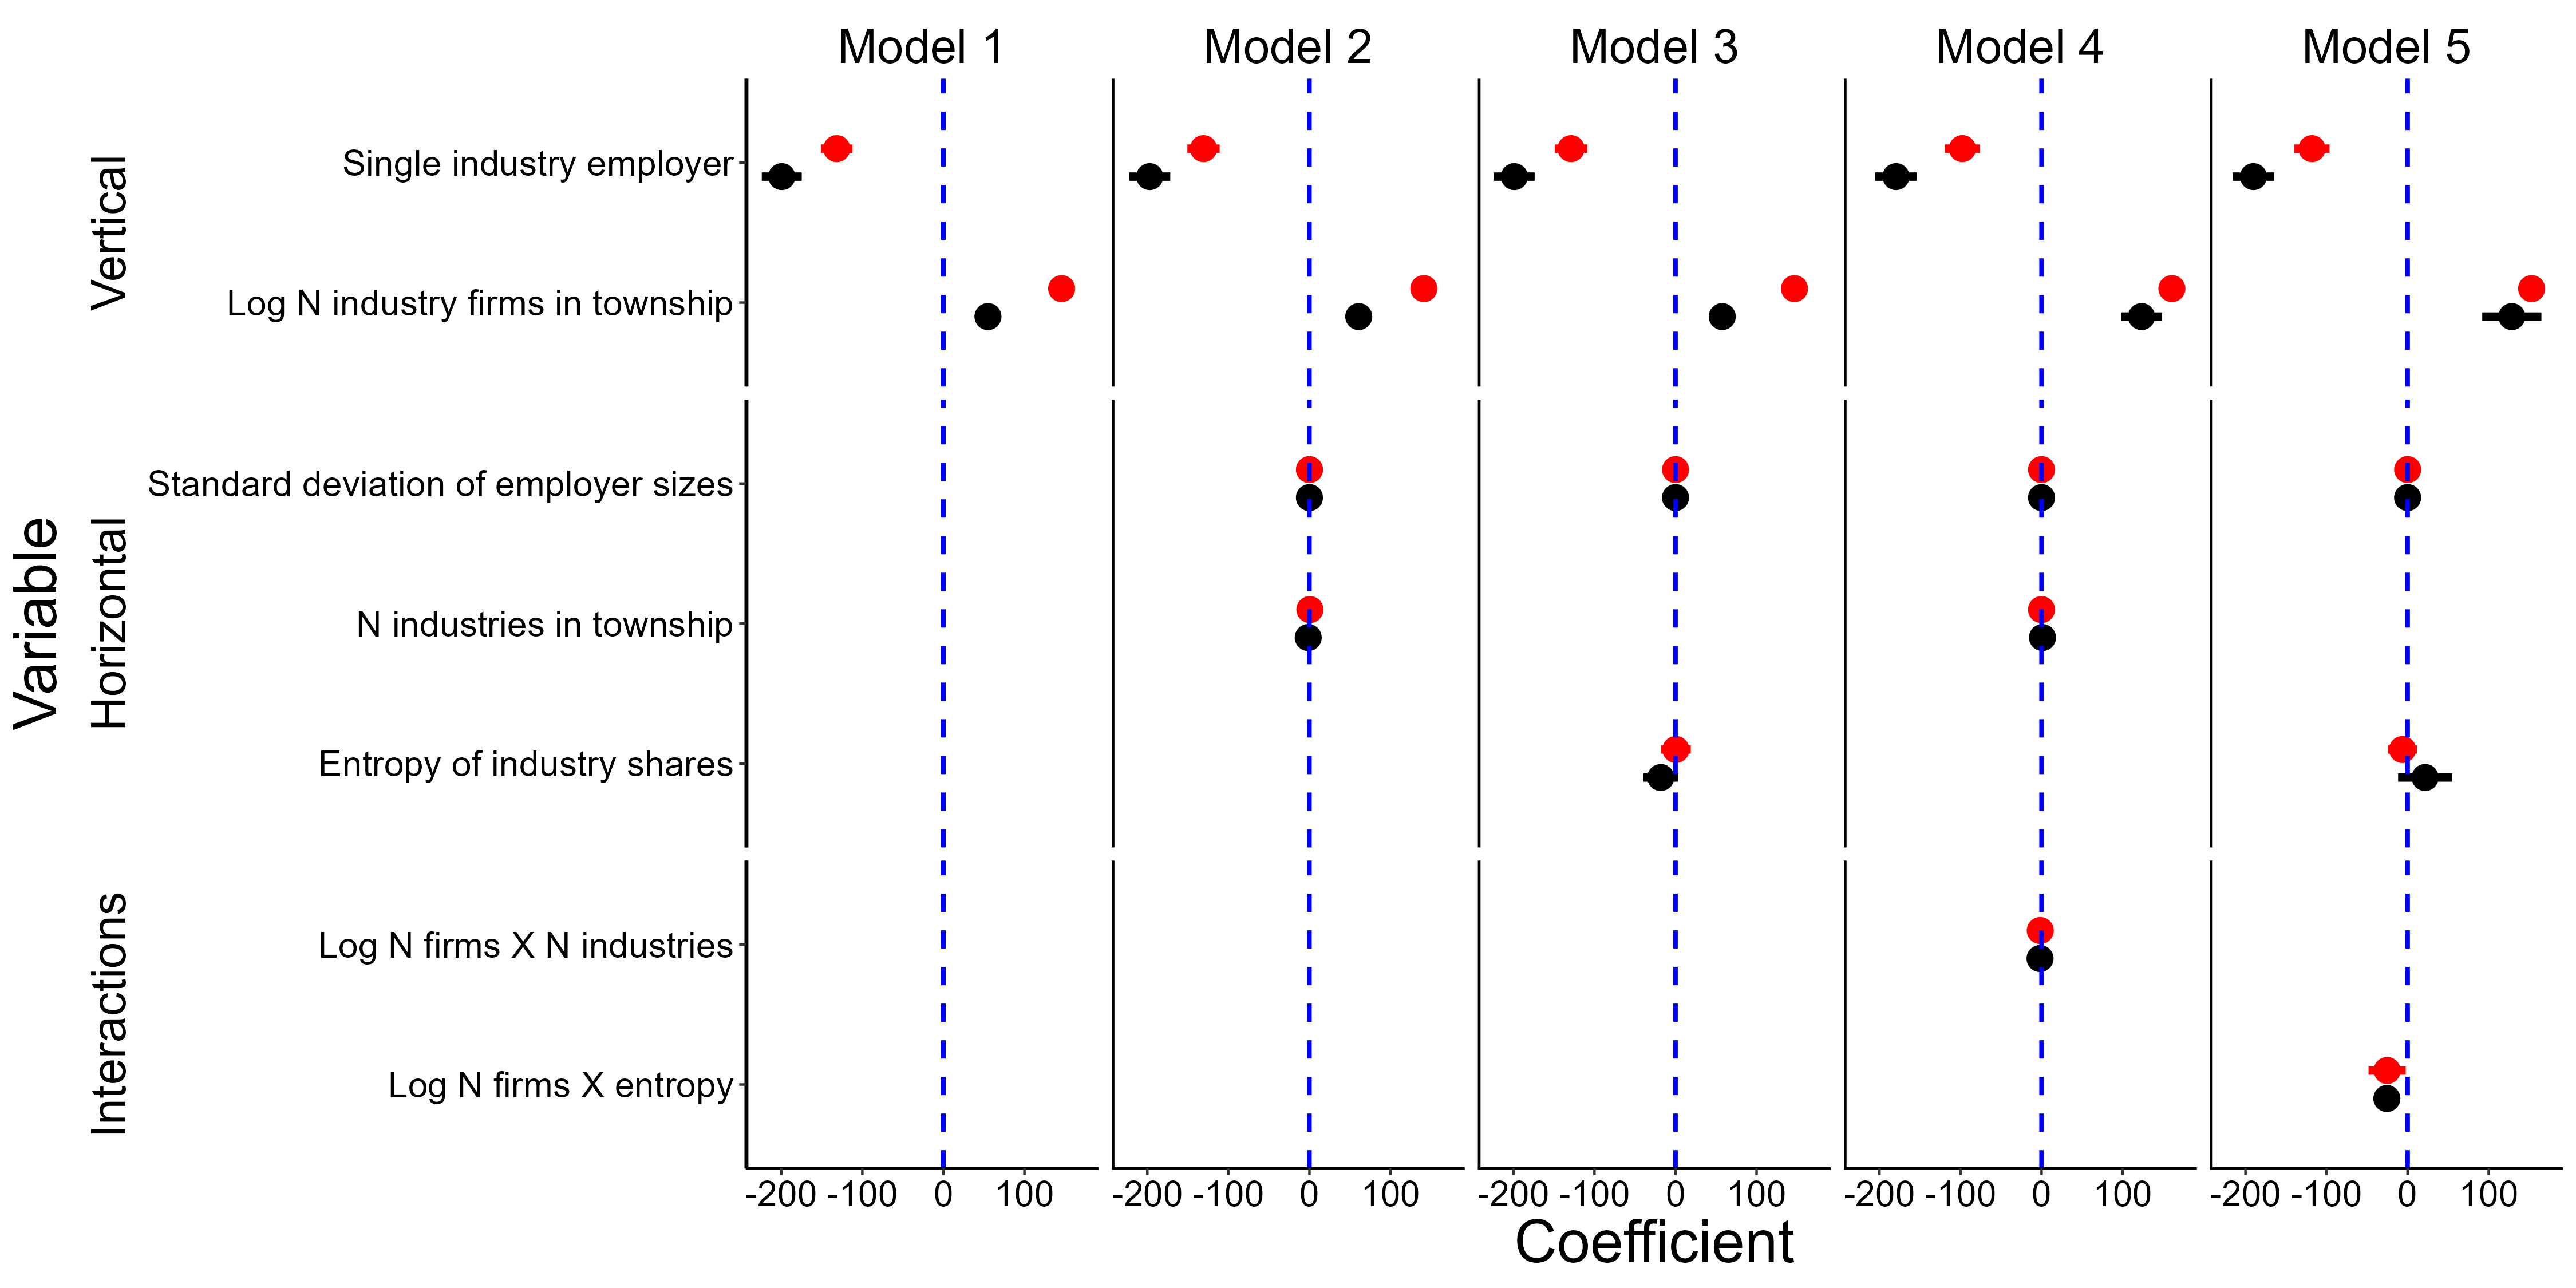
\includegraphics[width=1\textwidth]{grossvar_replication_1998_update.png}
\caption{Gross Income Dispersion.  Replication 1992-1998.}
\label{fig:gross_income}
\vspace{1cm} % Add some vertical space between the two images
  

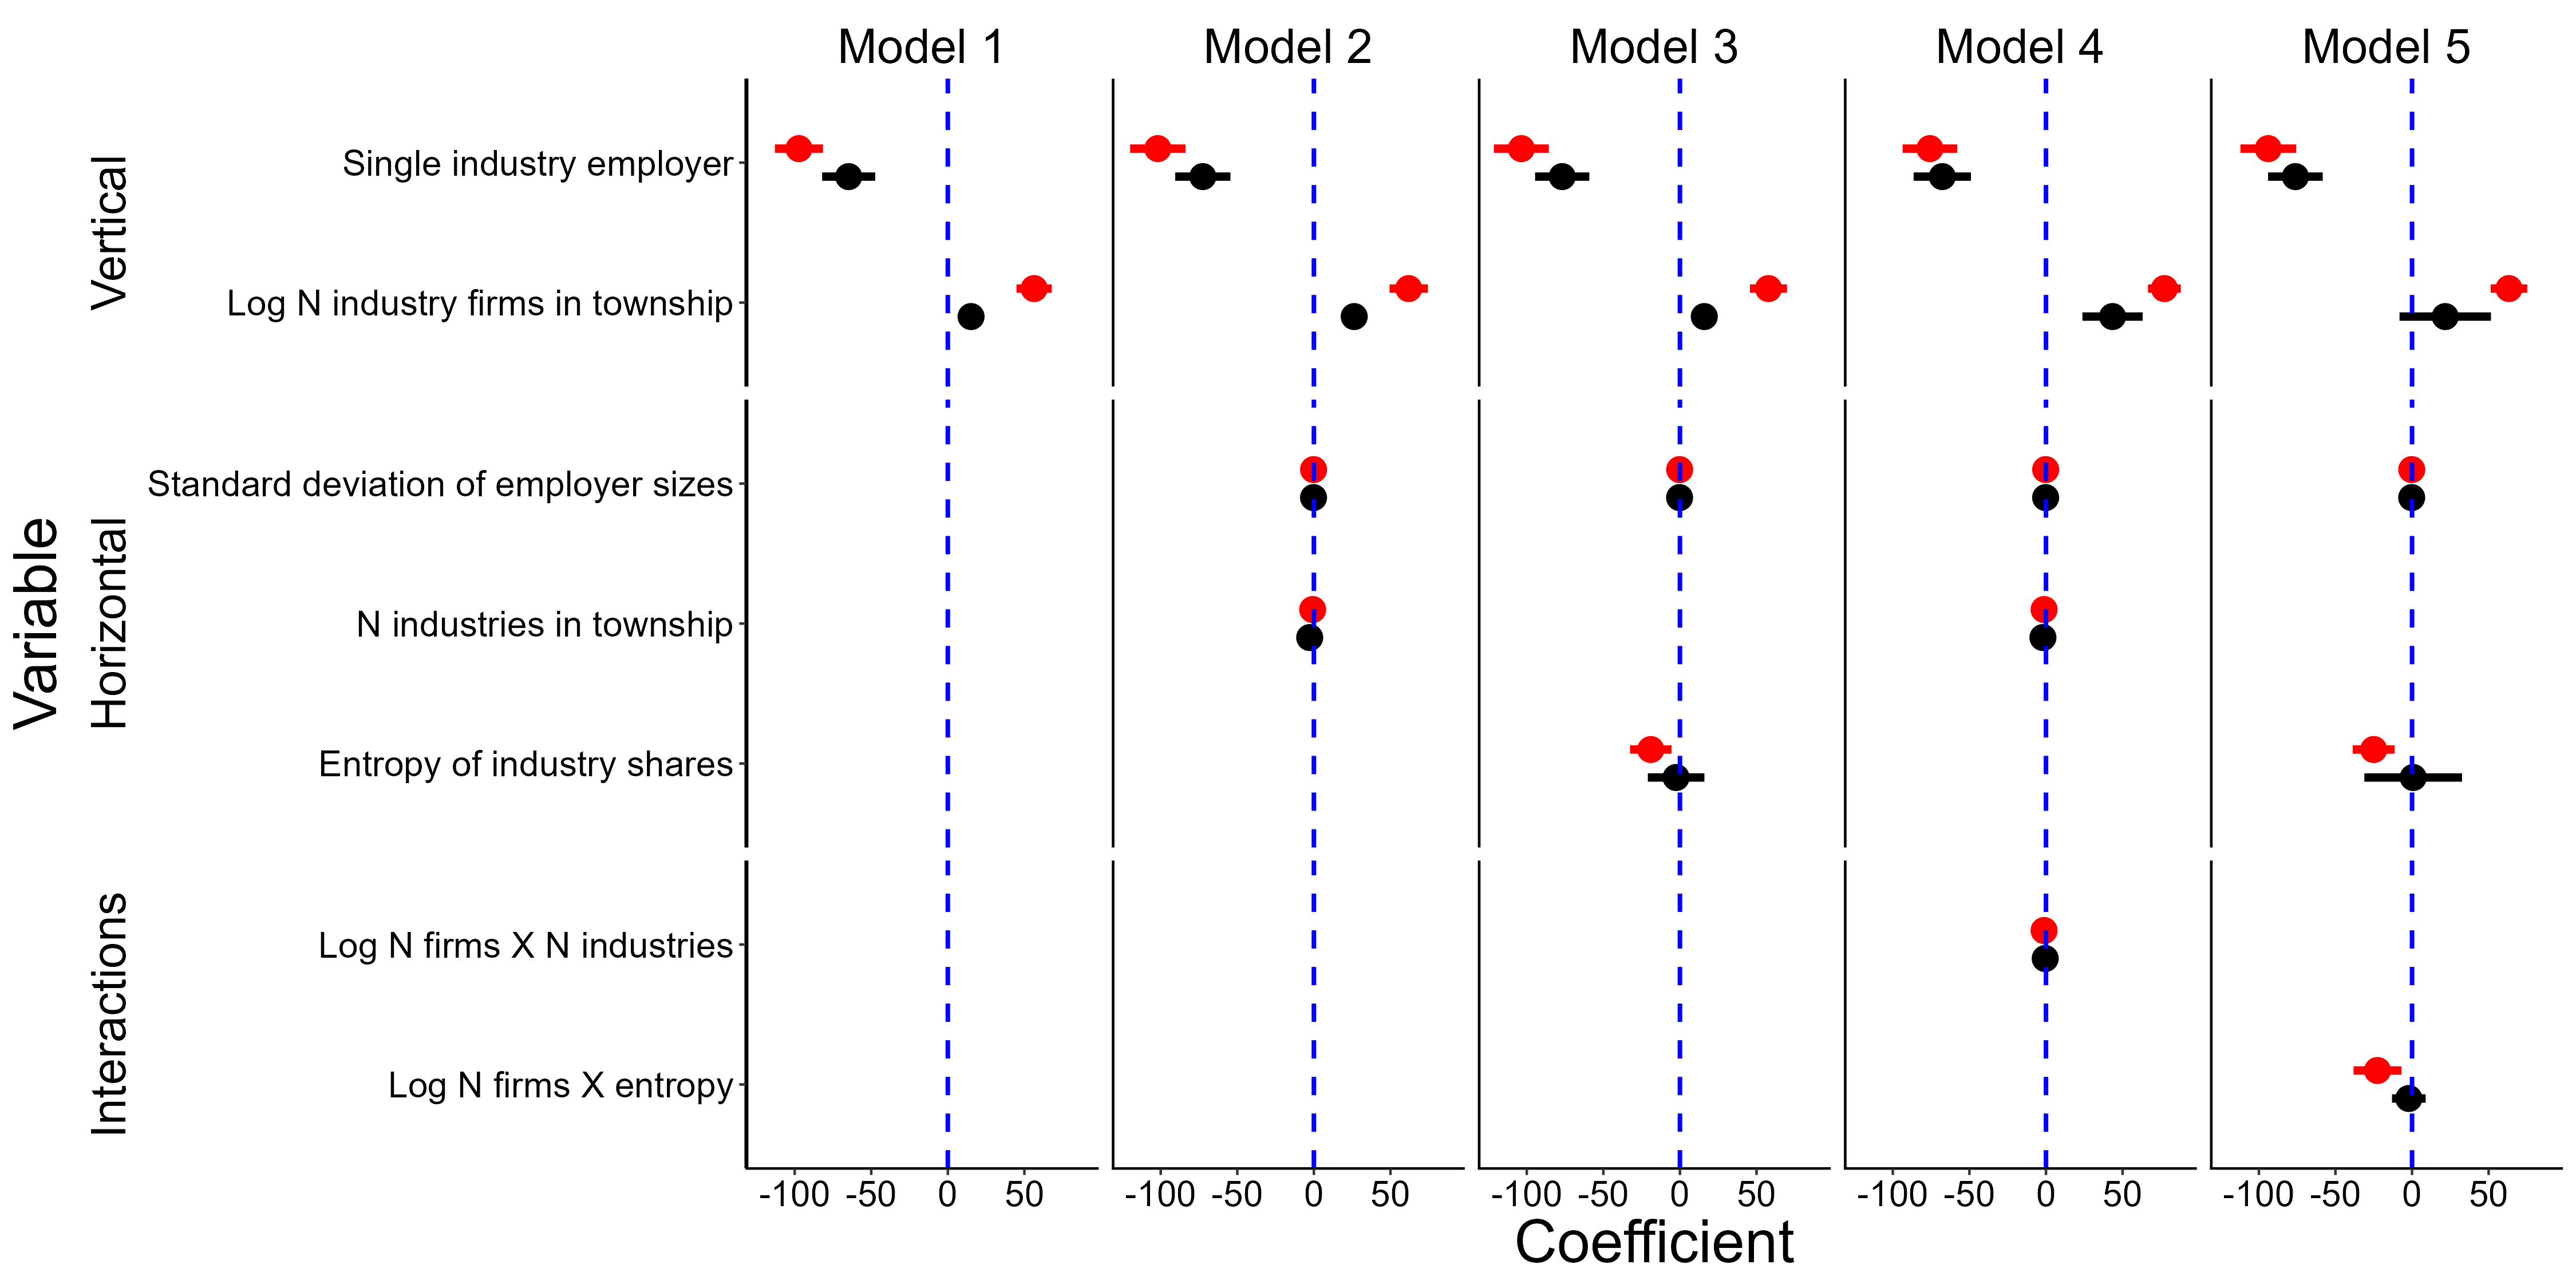
\includegraphics[width=1\textwidth]{resvar_replication_1998_update.png}
\caption{Residual Income Dispersion.  Replication 1992-1998.}  
\label{fig:residual_income}
\end{figure}


\clearpage % Start a new page
\thispagestyle{empty} % Remove page number from this page

\begin{figure}[htbp]
\centering
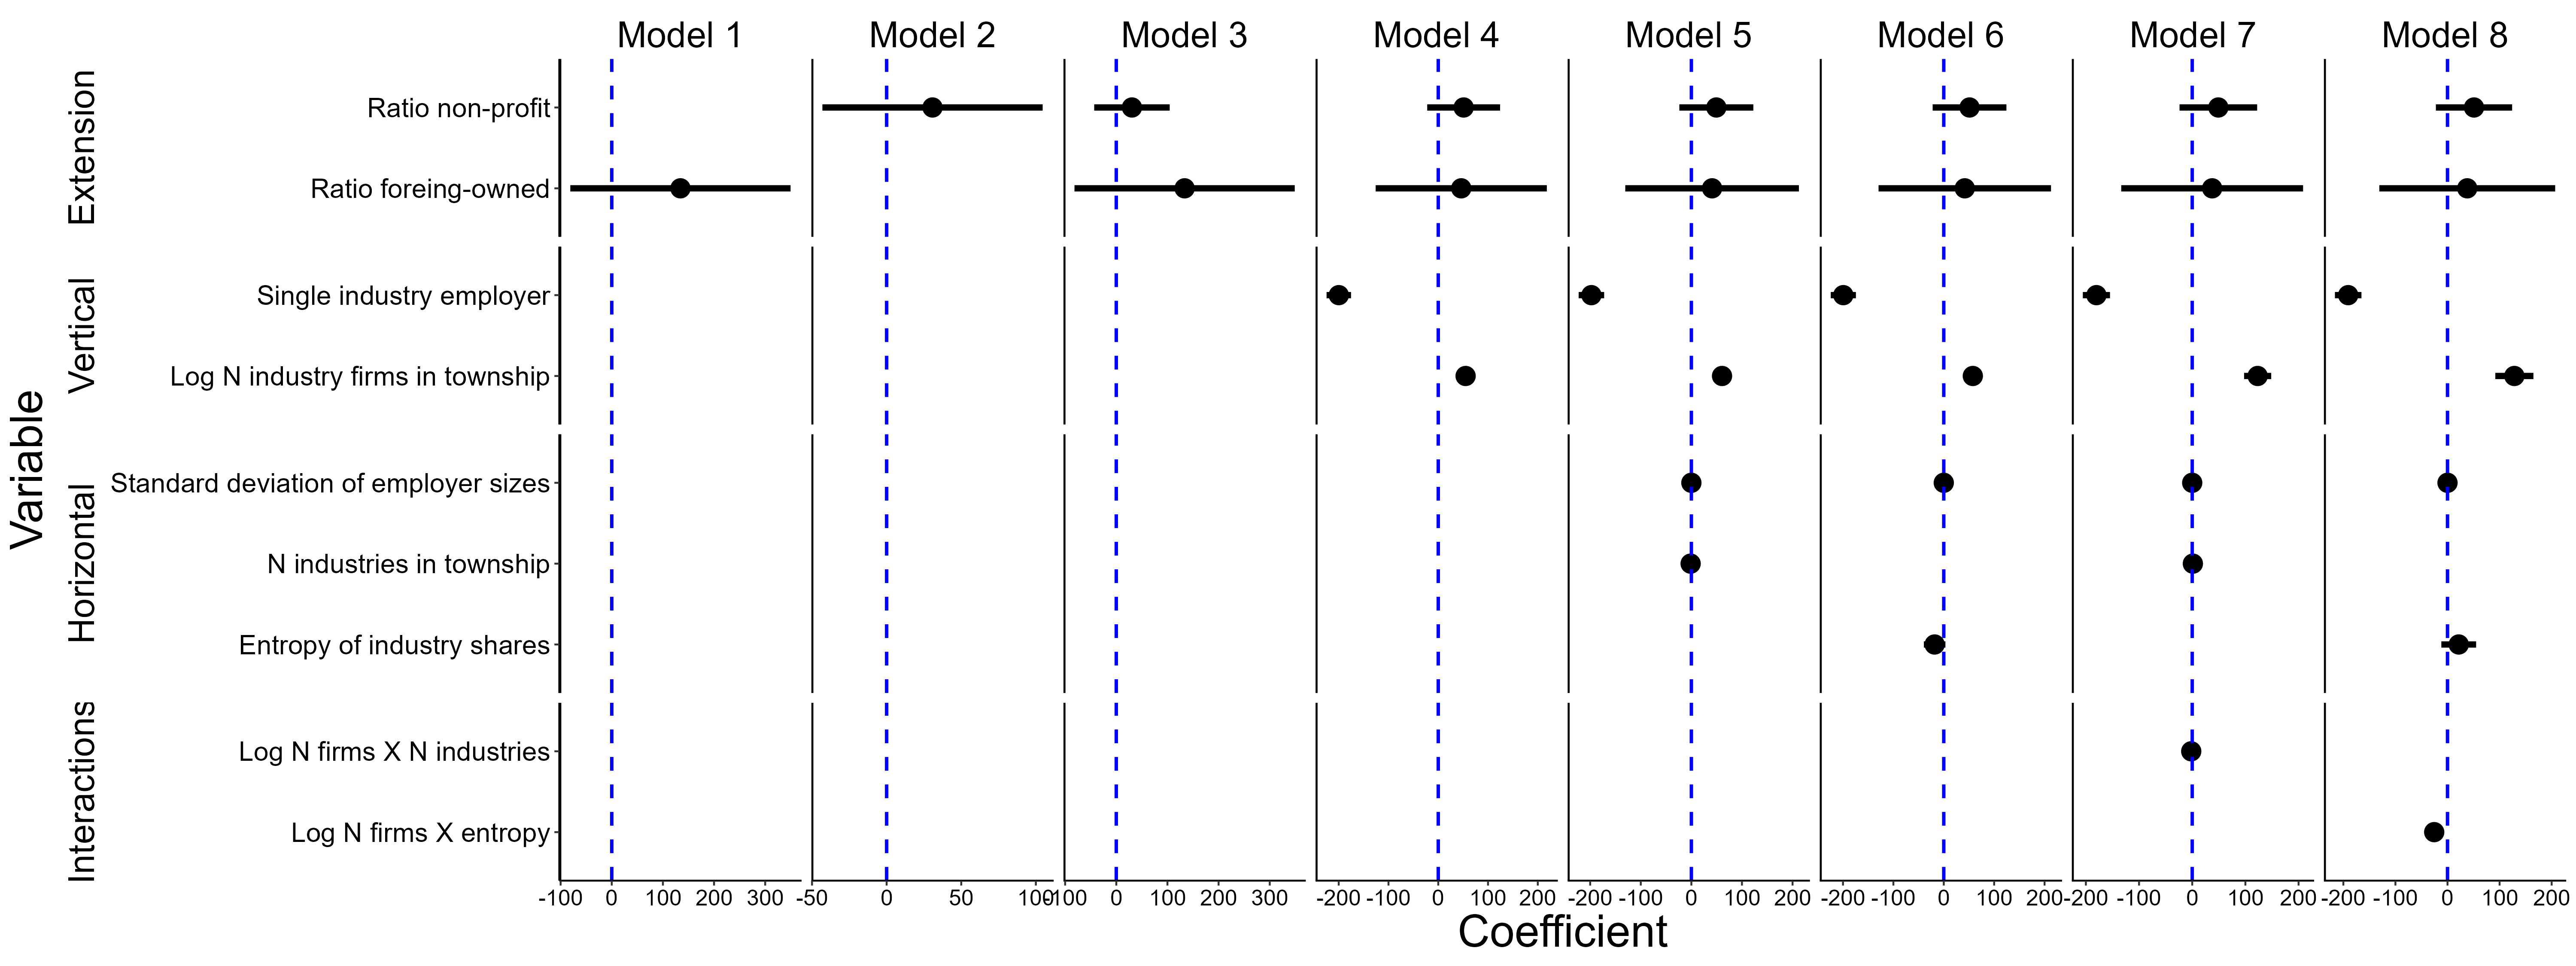
\includegraphics[width=1\textwidth]{grossvar_extension_1998_update.png}
\caption{Gross Income Dispersion.  Extension 1992-1998.}
\label{fig:gross_income}
  
  \vspace{1cm} % Add some vertical space between the two images

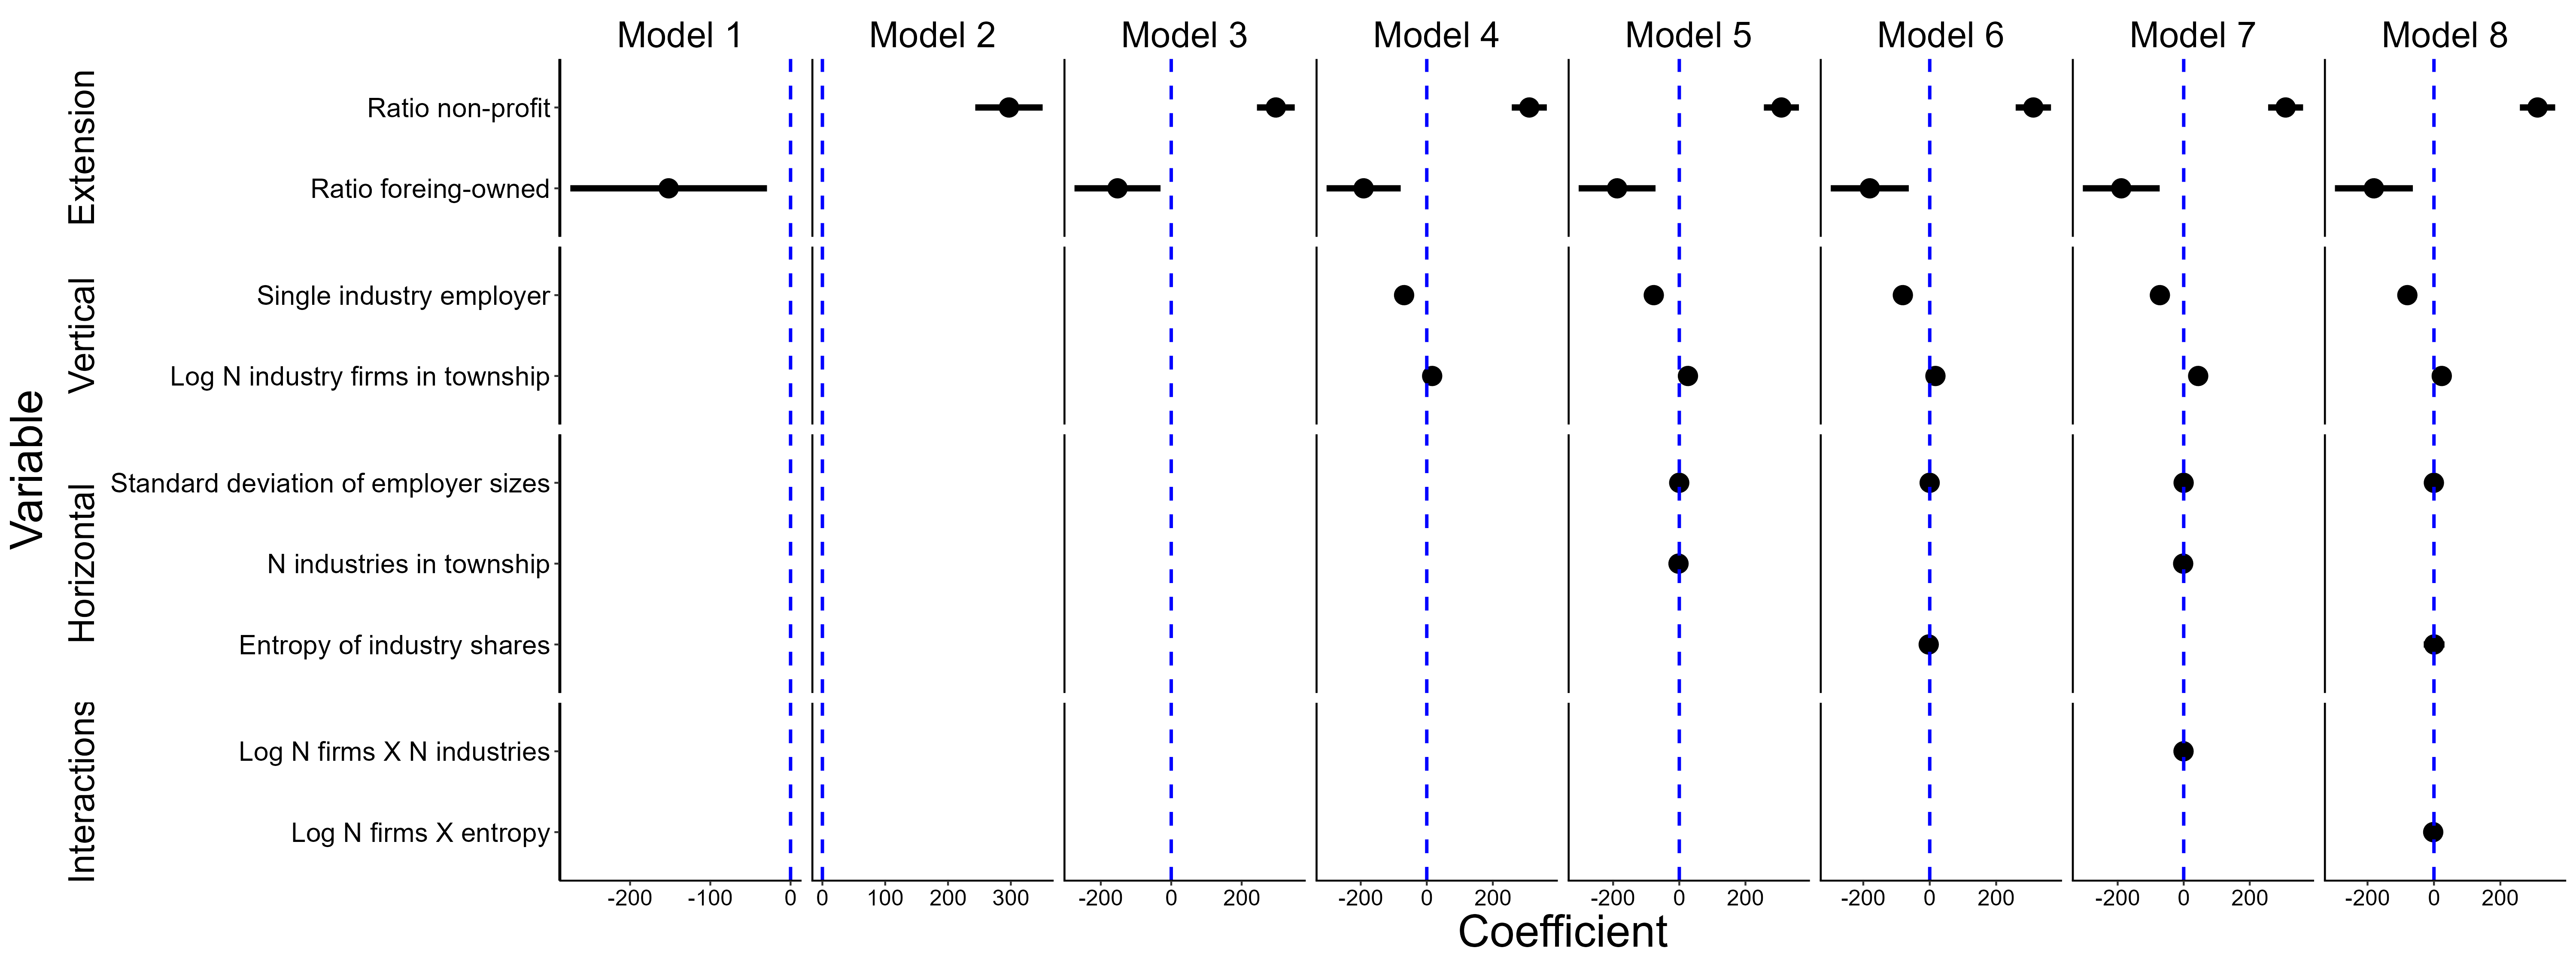
\includegraphics[width=1\textwidth]{resvar_extension_1998_update.png}
\caption{Residual Income Dispersion.  Extension 1992-1998.}  
\label{fig:residual_income}
\end{figure}




\clearpage % Start a new page
\thispagestyle{empty} % Remove page number from this page



\begin{table}[htbp]
\caption{Decisions and parameters for multiverse analysis}
\centering
\resizebox{\textwidth}{!}{%
\begin{tabular}{lp{4cm}p{4cm}p{4cm}}
\hline
%\multicolumn{4}{|l|}{\textbf{Header Row}} \\ \hline
\textbf{Decision} & \textbf{Description} & \textbf{S\&S decision}  & \textbf{Parameters}  \\ \hline
(1) Industries & Inclusion criteria for industries & S\&S excludes industries in agricultural and extractive & Omit industries in the agricultural and extractive industries or keep all sectors. \\ \\
(2) Sectors with public employees & Threshold for dropping industries with large public employee share (sensitivity analysis of S\&S 15 percent threshold).  & S\&S remove industries in which the public sector employed over 15 percent of the workforce & Omit industries where the public sector employed over a percent of the workforce, with thresholds: 0, 0.1, 0.15, 0.2, 0.3. \\ \\
(3) Wages & Omitting individuals with no income (but employed) and assess removal of individuals in lower-income brackets (to exclude part-time workers) & S\&S use hourly wage, thus, their analyses should be less sensitive to the influence from part-time workers  & Omit employees whose annual wage was below a certain threshold. Thresholds used: 0, 25 000, 50 000, 75 000, and 100 000 SEK. \\ \\
(4) Large organizations  & We omit large companies in several steps.  & S\&S do not exclude large firms   & Omit firms with more employees than a certain threshold. Thresholds used: 0, 500, 5 000, and 10 000 employees. \\ \\
(5) Workforce size & Number of smaller township deciles removed  & S\&S do not exclude townships based on their workforce size & Omit deciles of smallest townships in terms of workforce. Thresholds used: 0, 0.1, 0.2, 0.3, 0.4, and 0.5 \\ \hline

\multicolumn{4}{p{18cm}}{\textbf{Notes:} In deciding (1) cut-offs for Industrial codes, we use parameters that exclude industries related to agricultural and extractive as well as parameters that do not exclude them. For (2), we alternate the threshold for dropping industries with large public employee share in 10 percent intervals between 0 and 30 percent, as well as including S\&S decision on 15 percent. For (3), we omit employed individuals with no income and gradually remove individuals in lower-income brackets to exclude part-time workers (median wage in Sweden was 178,800 SEK in 1992 and 231,600 SEK in 1998). The main reason for this is that S\&S uses hourly wage whereas we use annual wage. For contextual factor (5), we omit large organizations above 500, 5000, or 10000 workers. We also include S\&S decision, i.e., not excluding firms based on their size. For contextual factor (6), we omit deciles from 0 to 0.5 of smallest townships in terms of workforce.} \\
\end{tabular}%
}
\label{tab:mytable}
\end{table}



\end{document}